\chapter{Introducción}

Implementar un transmisor de televisión digital, no es una tarea sencilla. El primer problema a enfrentar es el acceso a la información técnica. Existe poca documentación generada en el país, para cumplir con las condiciones técnicas de un sistema complejo y que, además, ya lleva 7 años de vigencia como oficial. La norma presentada por la ARIB deja varias zonas grises, asume por conocidos conceptos clave, y no se explaya mas de lo necesario en cuestiones de fondo. 

Existen fuertes limitaciones económicas para hacerse con software o hardware comercial que resuelvan incluso algunas de las funcionalidades que exige la norma. 

Esta tesis intenta suplir esa carencia, en principio complementando el trabajo iniciado por el grupo ARTES con el receptor \textit{gr-isdbt}. Se desarrolló a lo largo de este proyecto, un transmisor de televisión digital que cumple con las condiciones establecidas en la norma, y cuyas señales son decodificables por los televisores comerciales homologados por el LATU.

Contar con el trabajo presentado en \textit{gr-isdbt} fue una ayuda mayúscula, ya que el paradigma de código abierto permitió contrastar y testear los conceptos vertidos en la norma, lo que fue fundamental para la comprensión de que cosas sería necesario implementar para transmitir. Es fundamental para este grupo de trabajo destacar lo valioso de la generacion de proyectos de código abierto.

Esperamos contribuir con esta comunidad poniendo a disposición de cualquier persona el transmisor, para que continúen con el trabajo de aprendizaje, la optimización del mismo por técnicos y estudiantes con un mejor panorama del rubro del que tuvimos al implementar \textit{gr-isdbt-tx}.

Contribuir con la comunidad nacional de técnicos que trabajan en el rubro, y que no cuentan con documentacion técnica generada por y para la norma nacional, con los problemas y las particularidades que la transmisión tiene en nuestro país y no tener que abstraer de trabajos de terceros, que resolvieron problemas similares en contextos diferentes.

Existen en el Uruguay XX licencias de transmisión de televisión para el área nacional. Durante la implementación en el marco legal de la televisión digital, se entregaron 22 licencias para transmisión de televisión digital bajo la norma ISDBT. De ese total, solo algunos estan brindando el servicio de forma adecuada.

\begin{figure}
\centering
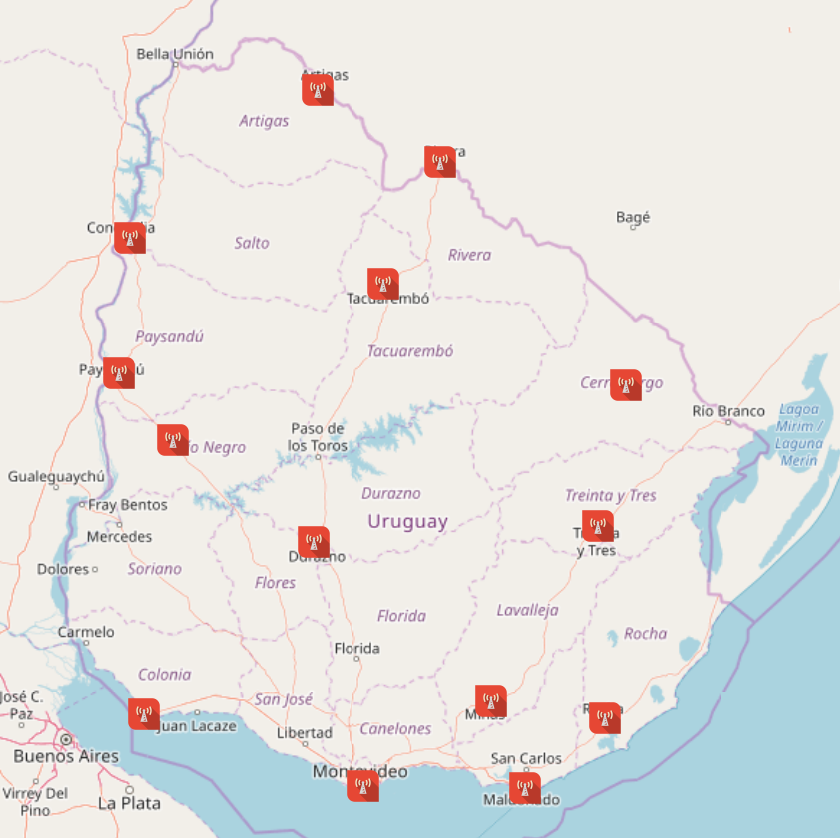
\includegraphics[scale=0.3]{figuras/cap01/mapa_estaciones}
\caption{\label{mapa_estaciones} Distribución de las estaciones transmisoras de TV digital en el Uruguay.}
\end{figure}

La situación de los consumidores del servicio tampoco es la ideal. La television analógica sigue siendo la mayor puerta de acceso al medio. La Encuesta Continua de Hogares del Instituto Nacional de Estadística\cite{ine2017}, cuyos indicadores son una muestra representativa de la situación de todos los hogares del país, dió a conocer que en el año 2017 solamente el 47 \% de los hogares encuestados tienen recepción a TV digital abierta. Tanto es asi, que el apagón analógico programado para 2015, fue postpuesto por tiempo indeterminado. En Argentina, la situación es similar, siendo postpuesto para 2019. El alto costo del recambio de equipamiento, y posturas sobre la democratización del acceso a la información para personas de bajos recursos, fundamentan estas decisiones.
	
Se logra visualizar el funcionamiento de la norma de televisión nacional, de forma mas clara y consisa de lo que habia actualmente. Los conceptos que deja la norma como documento se bajan a tierra en un formato de código abierto, y gratuito, lo que democratiza el acceso a la información que hoy por hoy existe mayoritariamente en hardware y software propietario con licencias caras.
	
Aparece la posibilidad de recrear una planta de transmisión de televisión nacional a muy bajo costo, permitiendo su reproducción tanto en el hogar por entusiastas, en el aula por docentes o en la industria, por tecnicos, lo cual puede colaborar con el mejoramiento de la calidad del servicio actual.
	
Sirve como ejemplo para algunos de los cursos de Facultad, generalmente denominados por el estudiantado como muy teóricos y con poco alcance práctico. 


Miren todo lo que aprendí, ver~\cite{Autor}.

